\documentclass[12pt, a4paper]{article}
\usepackage[brazil]{babel}
\usepackage[utf8]{inputenc}
\usepackage[T1]{fontenc}
\usepackage{times}
\usepackage{setspace}
\usepackage[margin=3cm]{geometry}
\usepackage{indentfirst}
\usepackage{graphicx}
\usepackage{hyperref}
\usepackage{subcaption} 
\usepackage{float}
\usepackage{amsmath} 
\usepackage{amssymb}

\onehalfspacing
\setlength{\parindent}{1.5cm}

\newcommand{\titulopt}{Fluxo óptico para análise de calçadas}
\newcommand{\tituloen}{Project Title}
\newcommand{\orientadores}{Roberto Marcondes Cesar Junior \\ Roberto Hirata Junior}
\newcommand{\processo}{ Chamada FAPESP Futuros Cientistas}

\begin{document}

\begin{titlepage}
    \begin{center}
        \large UNIVERSIDADE DE SÃO PAULO\\
        \large INSTITUTO DE MATEMÁTICA E ESTATÍSTICA\\[3cm]


        \textbf{\Large \titulopt}\\[2cm]
        
        
        \textbf{\large Renzo Real Machado Filho}\\[0.5cm]
        \centering \textbf{Orientadores:} \\
        \orientadores \\[3cm]
        
    
        \processo
        \vfill
        
        São Paulo \\ \today
    \end{center}
\end{titlepage}

\section*{Resumo}


\newpage
\tableofcontents
\newpage

\section{Introdução}

\section{Visão Computacional: Algoritmos e Aplicações \cite{szeliski2010}}

\subsection{Processamento de Imagens}

Nesse capítulo, trataremos do conjunto de operações e técnicas aplicadas a imagens digitais. É uma etapa de preparação para muitos algoritmos de reconhecimento de objetos, reconstrução 3D e/ou rastreamento de movimento. Nessa perspectiva, começaremos pelos chamados "operadores de ponto", que manipulam cada pixel de uma imagem, independentemente daqueles ao seu redor. Depois, passaremos pelos operadores "area-based", nos quais cada novo valor de um pixel depende de um certo número de pontos vizinhos.

Um operador genérico é uma função que toma uma ou mais imagens como inputs e produz uma outra imagem de output. Matematicamente,
\[
f(x) = h(g_0(x), \dots, g_n(x))
\]

Já uma imagem digital colorida é representado como uma matriz 3D (altura $\times$ largura $\times$ 3 canais). Os 3 canais são: Blue, Green, Red (em OpenCV é BGR).

\subsection{Operadores de Ponto}

\subsubsection{Transformações de Pixels}

\noindent\textbf{Ajuste de Brilho (Brightness) e Contraste (Contrast)} \\

\noindent\textbf{Tipo:} Transformação linear.

\noindent\textbf{Fórmula:} $ f(x) = a(x) \cdot g(x) + b(x) $, onde $a$ é dito o contraste e $b$, o brilho.

\noindent\textbf{Efeito:} O brilho desloca uniformemente todos os valores de pixel na imagem. Valores positivos clareiam a imagem, valores negativos escurecem. Enquanto isso, o contraste controla a diferença entre tons claros e escuros. Valores $> 1$ expandem a faixa tonal (aumentam o contraste), valores entre 0 e 1 comprimem a faixa tonal (reduzem o contraste).

\noindent\textbf{Quando usar:} Quando a imagem está muito escura ou muito clara globalmente ou quando a imagem está "chapada", i.e, sem muita variação tonal. \\

\noindent\textbf{Correção Gamma} \\

\noindent\textbf{Tipo:} Transformação não-linear.

\noindent\textbf{Fórmula:} $f(x) = g(x)^{1/\gamma}$.

\noindent\textbf{O que é Gamma ($\gamma$)?} É um parâmetro que define a curvatura da transformação não-linear aplicada aos valores de intensidade. Ele controla como os valores intermediários (tons médios) são mapeados, enquanto preserva os extremos (preto puro e branco puro). Por padrão, usa-se $\gamma \approx 2.2$.

\noindent\textbf{Efeito:} Se $\gamma > 1$, escurece os tons médios enquanto preserva pretos e brancos (aumenta contraste em tons escuros). Já $\gamma < 1$, clareia os tons médios enquanto preserva pretos e brancos (aumenta contraste em tons claros).

\noindent\textbf{Quando usar:} Para corrigir percepção visual ou problemas de iluminação não-lineares. \\

\noindent \textbf{Ordem das Operações} \\

Contraste/Brilho $\rightarrow$ Gamma

O Contraste/Brilho são lineares, trabalham no domínio da intensidade enquanto o Gamma é não-linear, trabalha no domínio perceptual. Se fizéssemos gamma primeiro a transformação linear posterior distorceria a curva gamma e os valores seriam re-escalados de forma inadequada, perdendo o controle preciso sobre a correção tonal.

\subsubsection{Color Balance}
Esse procedimento ajusta a intensidade relativa das cores primárias. A operação é feita por canal (R, G, B). Podemos multiplicá-los por um fator que altera seu brilho ou ainda operar sobre transformações mais complexas, como o mapeamento no espaço de cores XYZ. \\

\noindent\textbf{Espaço de Cores XYZ}\\

É um espaço de cor matematicamente definido, usando coordenadas tridimensionais (X, Y, Z) para descrever todas as cores visíveis ao olho humano.
\begin{itemize}
    \item \textbf{X:} Representa aproximadamente a sensibilidade ao vermelho
    \item \textbf{Y:} Representa o brilho luminoso (luminância)
    \item \textbf{Z:} Representa aproximadamente a sensibilidade ao azul
\end{itemize}

\subsubsection{Composição e Mascaramento (Compositing and Matting)}

Em muitos aplicativos de edição de fotos e de efeitos visuais, queremos inserir/combinar elementos em uma imagem. Esse processo é chamado de \textbf{composição} \cite{SmithAndBlinn:1996:BSM}.

Paralelo a isso, também é desejável extrair objetos de imagens, processo comumente chamado de \textbf{mascaramento}. Uma máscara define a área de uma imagem que deve ser mantida ou ignorada, permitindo que apenas certas partes da imagem sejam visíveis e sejam integradas com outros elementos \cite{Porter:1984:CDI, SmithAndBlinn:1996:BSM}. \\

\noindent \textbf{Alpha matting} \\

É um processo que visa estimar a translucidez de um objeto em uma determinada imagem. O "alpha matting" resultante descreve, em pixels, a quantidade de cores de primeiro e segundo plano que contribuem para a cor da imagem composta. \cite{germer2020fastmultilevelforegroundestimation} \\

\noindent \textbf{Alpha-Matted Color Image} \\

É uma imagem que além dos 3 canais de cor (RGB), possui um 4º canal intermediário (Alpha - $\alpha$) que representa:
\begin{itemize}
    \item $\alpha = 1$: Pixel totalmente opaco
    \item $\alpha = 0$: Pixel totalmente transparente
    \item $0 < \alpha < 1$: Pixel parcialmente transparente
\end{itemize}

Portanto, para compor uma nova imagem sobre uma imagem antiga, o \textit{over operator} é

\[
C = (1-\alpha) B + \alpha F
\]

A equação acima atenua a influência da imagem de fundo $B$ por um fator $(1 - \alpha)$ e,
em seguida, adiciona os valores de cor (e opacidade) correspondentes à camada de primeiro plano $F$.

\subsubsection{Equalização de Histograma}

O histograma de uma imagem é um gráfico que representa a frequência de cada nível de intensidade de cinza (ou cor) presente na imagem. Em uma imagem de 8 bits em escala de cinza, por exemplo, existem 256 níveis de intensidade, que vão de 0 (preto absoluto) a 255 (branco absoluto). O eixo horizontal do histograma representa esses níveis de intensidade, enquanto o eixo vertical indica o número de pixels que possuem cada uma dessas intensidades.

Imagens com baixo contraste tendem a ter seus histogramas concentrados em uma faixa estreita de valores. Por exemplo, uma imagem escura terá a maioria de seus pixels com valores de intensidade baixos, resultando em um histograma "amontoado" à esquerda. De forma análoga, uma imagem muito clara terá seu histograma concentrado à direita.

\begin{figure}[H]
    \centering
    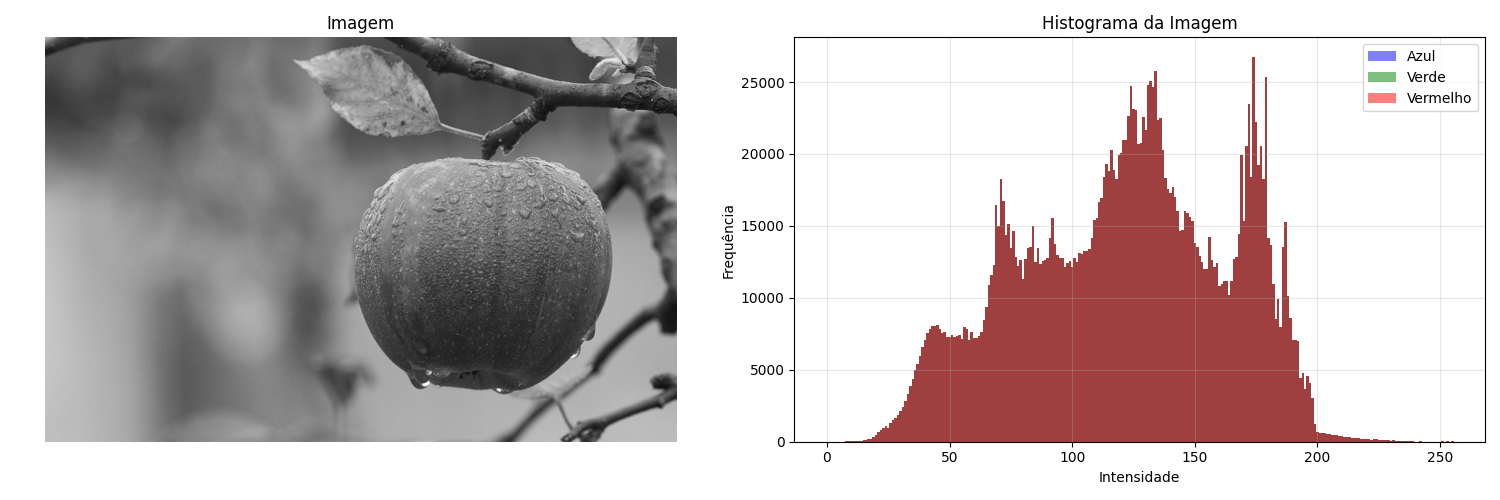
\includegraphics[width=1\linewidth]{Images/img+hist.png}
\end{figure}

\begin{figure}[H]
    \centering
    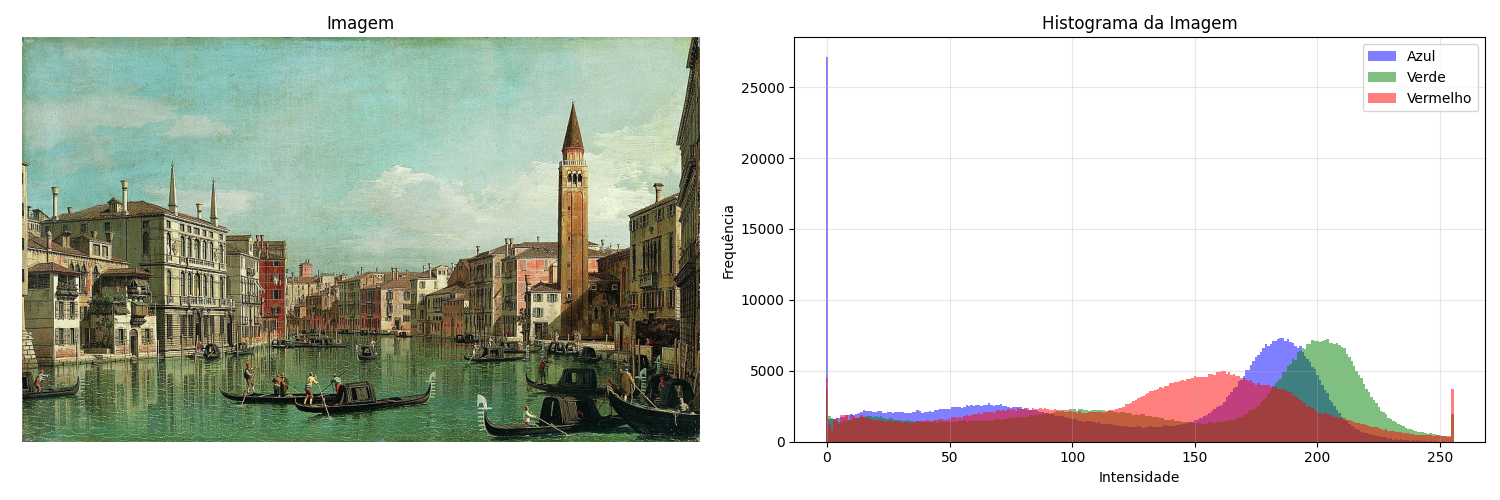
\includegraphics[width=1\linewidth]{Images/img+hist2.png}
\end{figure}

A equalização de histograma atua justamente nesse cenário, redistribuindo igualmente esses valores de intensidade por toda a gama possível. O objetivo é transformar o histograma original em um histograma mais próximo de uma distribuição uniforme, onde cada nível de intensidade tenha, idealmente, o mesmo número de pixels. Ao fazer isso, a diferença de intensidade entre os pixels é acentuada, o que melhora significativamente o contraste global da imagem.

Para isso, computamos a Função de Distribuição Acumulada (CDF), denotada por $c(I)$

\[
c(I) = \frac{1}{N}\sum_{i=0}^I h(i) = c(I-1) + \frac{1}{N}h(I),
\]

\noindent onde $I$ é o nível de intensidade atual (0-255 para imagens 8-bit), $h(I)$ é a frequência do nível de intensidade $I$ (valor do histograma) e $N$ é quantidade de pixels na imagem.

\section{Escala de Cinza}
O Cálculo da Escala de Cinza

Seu raciocínio de usar a média (R+G+B)/3 é perfeitamente lógico e seria a forma mais simples de fazer a conversão. No entanto, o método padrão é um pouco mais complexo, e o motivo é fascinante: a biologia do olho humano!

Nossos olhos não são igualmente sensíveis a todas as cores. Somos muito mais sensíveis à luz verde, um pouco menos à vermelha e bem menos à azul.

Para criar uma representação em escala de cinza que pareça "natural" para um ser humano em termos de brilho percebido, a conversão usa uma média ponderada. Os canais de cor que percebemos melhor têm um peso maior no cálculo final.

A fórmula padrão (usada pelo OpenCV e em muitas outras aplicações) é:

$Y=0.299R + 0.587G + 0.114B$

Onde Y é o valor do pixel de luminância (o valor de cinza).

Veja como o Verde (G) tem um peso enorme (quase $60\%$), enquanto o Azul (B) tem um peso bem pequeno. Isso garante que uma imagem com muito verde pareça mais clara em escala de cinza do que uma imagem com muito azul, o que corresponde à nossa percepção.


\section{Fluxo Óptico}

O fluxo óptico é definido como a distribuição das velocidades aparentes do movimento dos padrões de brilho em uma imagem. \cite{Horn1981}. 

\subsection{Campo de Movimento (Motion Field)}

Trata-se da velocidade de um ponto que se move na cena/imagem. Em muitos casos, esse conceito se confunde com o fluxo óptico. 

\subsection{\textit{Optical Flow Constraint Equation}}

Suponha que temos um ponto $(x,y)$ numa imagem que se moveu para $(x+\delta x, y+\delta y)$. O seu  deslocamento é $(\delta x, \delta y)$ e queremos medir esse movimento. Dizemos que o fluxo óptico é $(u, v) = (\frac{\delta x}{\delta t}, \frac{\delta y}{\delta t})$ num tempo $\delta t$, pequeno. \\

\textit{Suposição 1:} O brilho de um ponto é constante ao longo do tempo. Então, 

\[ I(x, y, t) = I(x+ \delta x, y + \delta y, t+\delta t).\]

\textit{Suposição 2:} O deslocamento $(\delta x, \delta y)$ e o passo $\delta t$ são pequenos. \\

Com isso, por Taylor, temos

\[ f(x+\delta x) = f(x) + \frac{\partial f}{\partial x} \delta x + \dots + \frac{\partial^n f}{\partial x^n} \frac{\delta x^n}{n!}\]

Se $\delta x \to \infty$, então $f(x + \delta x) = f(x) + \frac{\partial f}{\partial x} \delta x + O(\delta x^2)$.

Para $\delta x, \delta y$ e $\delta t$ suficientemente pequenos, vale que

\[ f(x + \delta x, y + \delta y, t + \delta t) \approx f(x, y, t) + \frac{\partial f}{\partial x} \delta x + \frac{\partial f}{\partial y} \delta y + \frac{\partial f}{\partial t} \delta t \]

Pela \textit{suposição 2}, temos

\[ I(x + \delta x, y + \delta y, t + \delta t) = I(x, y, t) + I_x \delta x + I_y \delta y + I_t \delta t\]

Pela \textit{suposição 1} e subtraindo ambas as equações, obtemos

\[ I_x \delta x + I_y \delta y + I_t \delta t = 0\]

Dividindo por $\delta t$ e com $\delta t \to 0$, temos

\[ I_x \frac{\delta x}{\delta t} + I_y \frac{\delta y}{\delta t} + I_t  = 0\]
\[ \Leftrightarrow I_x u + I_y v + I_t  = 0, \]

onde $(u, v)$ é o fluxo óptico.

\subsubsection{Problema da Abertura}

\subsection{O método de Lucas-Kanade}

Vimos que, pelo resultado anterior, a equação de restrição de fluxo óptico é um problema mal posto. Assim, é necessário mais uma suposição. \\

\textit{Suposição 3:} para cada pixel, assuma que o campo de movimento e o fluxo óptico são constantes em uma pequena vizinhança $W$.

Para quaisquer $(l,k) \in W$, vale

\[ I_x(l,k) u + I_y(l,k) v + I_t(l,k)  = 0 \]

Isso resulta em um sistema de equações. Logo, na forma matricial para $W_{n\times n}$, temos

\[
\underbrace{
\begin{bmatrix}
I_x(1,1) & I_y(1,1) \\
\vdots & \vdots \\
I_x(n,n) & I_y(n,n)
\end{bmatrix}
}_{A}
\underbrace{
\begin{bmatrix}
u \\
v
\end{bmatrix}
}_{x}
=
\underbrace{
\begin{bmatrix}
I_t(1,1) \\
\vdots \\
I_t(n,n)
\end{bmatrix}
}_{B}
\]

Esse é um clássico problema do tipo $Ax=B$. Portanto, podemos resolvê-lo por mínimos quadrados, obtendo

\[
x = (A^T A)^{-1}A^TB.
\]

\subsubsection{Condições}

\begin{itemize}
    \item $A^TA$ deve ser inversível
    \item $A^TA$ deve estar bem condicionada:
    \begin{itemize}
        \item Sejam $\lambda_1, \lambda_2$ os autovalores de $A^TA$. Então, $|\frac{\lambda_1}{\lambda_2}| \approx 1$ e $\lambda_1, \lambda_2 > \epsilon$.
    \end{itemize}
\end{itemize}

As seguintes situações descrevem situações comuns: \\

\textbf{Regiões Homogêneas}

Regiões sem muita textura dificultam a visualização de movimento. Matematicamente, $\lambda_1 \approx \lambda_2$, mas ambos são pequenos. \\

\textbf{Bordas}

Regiões com presença de bordas geram um problema mal condicionado. Os gradientes estão predominantemente em um direção, i.e, a variação significativa está em uma única direção. Assim, o resultado da estimação de fluxo óptico pode ser ambíguo. Matematicamente, $\lambda_1 >>> \lambda_2$. \\

\textbf{Regiões Texturizadas}

Nesse cenário, a estimativa é muito boa. Há muitas variações nos padrões de brilho. Matematicamente, $\lambda_1 \approx \lambda_2$ e $\lambda_1, \lambda_2 > \epsilon$.

\subsection{Coarse-To-Fine Flow Estimation (Estimação de Fluxo do "Grosso ao Fino") }

Quando temos uma sequência de imagens com grandes movimentos, a aproximação por série de Taylor não é mais válida, bem como suas suposições.


\section{State-of-Art}

A estimação de movimento nas cenas pode ser dividido em três métodos: knowledge-driven, data-driven e hybrid-driven. 

\subsection{knowledge-driven}

É baseado em suposições para restringir o processo de estimação e modelar a correspondência espacial-temporal. Os primeiros métodos são Horn e Schunck (HS) e Lucas e Kanade (LK). 

\subsubsection{Desafios}

\textbf{Grandes Deslocamentos}

Objetos que se movem em rapidamente producem grandes distâncias entre os pixels nas cenas, o que dificulta o cálculo. Para lidar com esse problema, é usual utilizar uma estratégia "fino ao grosso" (coarse-to-fine).

\textbf{Oclusão}

A oclusão é o processo de detectar e/ou rastrear objetos quando estão ocultos ou obstruídos numa cena. Os métodos mais comuns adotam um esquema de verificação de consistência.

\textbf{Variações de Iluminação}

A clássica suposição de constância do brilho não se aplica em contextos de mudanças de iluminação. ???

\textbf{Ruído}

Filtros são aplicados em um campo para reduzir o ruído e melhorar a qualidade do mapeamento do fluxo.

\subsection{Data-driven}

As técnicas mais dominantes utilizam o deep learning. As CNNs tem sido muito bem sucedidas para a estimação de fluxo óptico. Por sua vez, esses métodos se dividem em U-Net e em Rede de Pirâmide Espacial.

Comumente, os métodos data-driven usam um ground truth como um sinal supervisionado, o que depende de dados rotulados. Entretanto, coletar um ground truth denso a nivel de pixel para cenas reais é um processo complicado e longo.

\subsubsection{U-Net}

Utiliza a estrutura de encoder-decoder. Por causa da contração e expansão do mapeamento de features nos encoders e decoders, há perda de detalhes importantes, o que é prejudicial para a estimação densa de movimento e atrapalha a acurácia e o detalhamento do campo de fluxo.

\subsubsection{Rede de Pirâmide Espacial}

O SPyNet foi a primeira arquitetura a utilizar essa técnica, cuja principal vantagem é o tamanho reduzido do modelo. Entretanto, sua acurácia ainda não pe capaz de bater o FlowNet2.0. O SPyNet estima grandes movimentos na camada mais grossa e deforma a segunda imagem em direção ao primeiro usando o fluxo amostrado de um nível anterior.

Esse mecanismo tem a característica de ser muito "personalizável" para a estimação de fluxo óptico. Sua construção detém diversos princípios da área, como a pirâmede espacial, deformação (warping) e pós-processamento. Isso é capaz de aumentar muito a eficiência e a acurácia da técnica.

\subsection{Hybrid driven}

Tais métodos usam suposições téoricas e, também, dados não-rotulados para o treino.

\subsubsection{U-Net e Rede de Pirâmide Espacial}

Para contornar o problema dos dados, vários trabalhos tentam aprender de maneira não supervisionada baseando-se em suposições teóricas. Outros tentam trabalhar de forma semi-supervisionada. Todavia, ainda não foram capazes de obter acurácias melhores nos mesmos datasets públicos.

\subsection{Métricas}

\subsubsection{End-to-End Point Error (EPE) and Average Endpoint Error (AEE)}

O erro de ponto final (EPE) para um determinado pixel ou ponto é calculado como a distância euclidiana entre o vetor de fluxo óptico estimado e o vetor de fluxo óptico da verdade básica naquele local.

O erro médio do ponto final (AEE), que calcula a distância euclidiana entre o campo de fluxo calculado e o campo de fluxo da verdade básica. Com isso, é nada mais que a média entre todos os pontos/pixels do cálculo anterior.

\[ \frac{1}{HW} \sum \underbrace{\sqrt{(u_* - u)^2 + (v_* - v)^2}}_{EPE}\hspace{0.2cm}, \]

onde $HW$ é número total de pixels na imagem, $(u_*, v_*)$ o ground truth e $(u,v)$ a estimativa do fluxo óptico.

\subsubsection{Average Angular Error (AAE)}

Para cada pixel, o erro angular é o ângulo entre o vetor de fluxo estimado e o vetor de fluxo do ground truth. Isso mede a precisão direcional do movimento estimado.

O AAE é a média desses erros angulares individuais em todos os pixels da imagem ou em uma região específica de interesse. Ele fornece um único valor que indica a precisão direcional geral do algoritmo de fluxo óptico.

\[ \frac{1}{HW} \sum \arccos \Bigg( \frac{u_*u + v_*v + 1}{\sqrt{(u_*^2 + v_*^2 +1)(u^2 + v^2 + 1)}}\Bigg) \]

\subsubsection{Root-Mean-Square Error (RMSE)}

Quantifica a precisão da estimativa de movimento. O valor do RMSE é expresso em pixels por quadro (px/frame). Se o RMSE for 1.5, significa que, em média, a ponta do vetor estimado está errada por 1.5 pixels em relação à ponta do vetor correto.

Quanto menor, melhor. Um RMSE baixo indica que os vetores estimados estão muito próximos dos vetores reais. Isso significa que o algoritmo é preciso. Quanto maior, pior. Um RMSE alto indica que há uma grande discrepância entre o movimento estimado e o movimento real. O algoritmo tem baixa precisão.

\[ \sqrt{1/HW \sum_{(x,y)} (I_{\text{warped}} (x,y) - I(x,y))^2 } \hspace{0.2cm} ,\]

onde $I(x, y)$ é a intensidade do pixel na posição $(x, y)$ do segundo quadro (o quadro para o qual estamos tentando prever o movimento) e $I_{\text{warped}}(x, y)$ é a intensidade do pixel na posição (x, y) da imagem warpeada.

\textbf{Limitações:} Um RMSE baixo pode ser causado por uma performance excelente em 90\% da imagem, mas um desempenho terrível em 10\% (e.g., em regiões de oclusão). A média pode mascarar esses erros localizados.

O RMSE mede principalmente a magnitude do erro. Dois vetores que apontam para direções completamente opostas, mas com magnitudes similares, podem ter um erro de magnitude pequeno, embora o erro de direção seja catastrófico. Por fim, a métrica só é válida se você tiver um ground truth confiável.

\subsubsection{Outliers ou Pontos Ruins}

Embora a média do EPE (AEE) seja uma métrica útil, ela pode ser distorcida por erros muito grandes em poucas regiões da imagem. Para contornar isso, define-se o conceito de \textbf{outlier}, que é uma predição considerada um erro grave. Em benchmarks de referência, como o KITTI, um pixel é classificado como outlier se o seu erro satisfizer a seguinte condição:

\[ \text{EPE} > 3 \text{ pixels} \quad \text{E} \quad \text{EPE} > 0.05 \cdot || {v}_{\text{gt}}|| \]

Esta condição dupla estabelece um limiar de erro absoluto (3 pixels) e um limiar de erro relativo (5\% da magnitude do vetor ground truth), tornando a avaliação mais robusta para diferentes magnitudes de movimento.

\subsubsection{Fl-all}

A métrica F1-all (Flow outliers averaged over all pixels) indica a porcentagem de "pontos ruins" (outliers), onde um "ponto ruim" satisfaz as equações na seção anterior. Assim, temos

\[ Fl-all = \frac{N}{HW} \times 100\%\]

\subsection{Datasets}

\subsubsection{MPI Sintel}
Derivado da animação de código aberto "Sintel", este é um dataset sintético desafiador que inclui cenas complexas e fotorrealistas. É um dos benchmarks mais importantes para avaliação de algoritmos de fluxo óptico.
\begin{itemize}
    \item \textbf{Conteúdo:} Cenas com movimentos amplos, desfoque de movimento (\textit{motion blur}), oclusões, superfícies não lambertianas (reflexos) e efeitos atmosféricos (névoa, fumaça).
    \item \textbf{Ground Truth:} Fornece fluxo óptico denso e preciso.
    \item \textbf{Versões:} Possui duas versões para avaliação: \textbf{Clean}, que contém as cenas com renderização padrão, e \textbf{Final}, que adiciona desfoque de movimento e efeitos atmosféricos, tornando a estimação mais difícil.
    \item \textbf{Uso Principal:} Avaliação (benchmark) de algoritmos em condições complexas e variadas.
\end{itemize}

\subsubsection{KITTI}
O dataset KITTI é composto por sequências de vídeo do mundo real, capturadas a partir de um carro em movimento em ambientes urbanos e rodoviários. É o benchmark padrão para tarefas de visão computacional relacionadas à condução autônoma.
\begin{itemize}
    \item \textbf{Conteúdo:} Cenas de rua, com carros, pedestres e edifícios. Inclui dados de múltiplos sensores, como câmeras estéreo, Lidar e GPS/IMU.
    \item \textbf{Ground Truth:} O fluxo óptico é \textbf{esparso}, gerado a partir da projeção de dados 3D do Lidar nas imagens. Apenas pixels com correspondência 3D confiável possuem ground truth.
    \item \textbf{Versões:} Os benchmarks de fluxo óptico mais comuns são o KITTI 2012 e o KITTI 2015.
    \item \textbf{Uso Principal:} Avaliação de algoritmos em cenários de condução autônoma do mundo real.
\end{itemize}

\subsubsection{FlyingThings3D}
Um dataset sintético de grande escala, projetado especificamente para treinar redes neurais profundas. Ele apresenta uma vasta gama de objetos e movimentos.
\begin{itemize}
    \item \textbf{Conteúdo:} Objetos do cotidiano (extraídos do dataset ShapeNet) que se movem em trajetórias 3D aleatórias sobre fundos variados.
    \item \textbf{Ground Truth:} Fornece fluxo óptico denso e mapas de disparidade estéreo.
    \item \textbf{Características:} Destaca-se pelo seu tamanho massivo e pela grande variedade de movimentos, o que ajuda na generalização dos modelos.
    \item \textbf{Uso Principal:} Treinamento em larga escala de modelos de aprendizado profundo para fluxo óptico e estéreo.
\end{itemize}

\subsubsection{FlyingChairs}
Foi um dos primeiros datasets sintéticos de grande escala criados para o treinamento de redes convolucionais para fluxo óptico (notavelmente, o FlowNet). É conceitualmente mais simples que o FlyingThings3D.
\begin{itemize}
    \item \textbf{Conteúdo:} Imagens de modelos 3D de cadeiras renderizadas e sobrepostas a imagens de fundo aleatórias do Flickr. As cadeiras e os fundos são movidos usando transformações afins 2D aleatórias.
    \item \textbf{Ground Truth:} Fornece fluxo óptico denso e preciso.
    \item \textbf{Uso Principal:} Pré-treinamento ou treinamento inicial de redes neurais para a tarefa de estimação de fluxo óptico, devido à sua simplicidade e tamanho.
\end{itemize}

\subsubsection{Middlebury}
Este é um dataset clássico, composto por cenas de laboratório do mundo real, capturadas em alta resolução e sob condições de iluminação controladas.
\begin{itemize}
    \item \textbf{Conteúdo:} Cenas internas com texturas ricas e movimentos geralmente pequenos e bem definidos.
    \item \textbf{Ground Truth:} Fluxo óptico denso e de altíssima precisão, obtido com técnicas avançadas que não são aplicáveis em cenários gerais.
    \item \textbf{Características:} Devido ao seu tamanho reduzido, não é adequado para treinamento. Seu foco é a avaliação da \textbf{precisão} dos algoritmos em condições quase ideais.
    \item \textbf{Uso Principal:} Benchmark de alta precisão para comparar a acurácia de diferentes métodos de fluxo óptico.
\end{itemize}



\bibliographystyle{IEEEtran}
\bibliography{refs}

\end{document}